\section{Abschluss}
An diesem Punkt ist die prototypische Implementierung der aufgebauten Hybrid-Cloud-Architektur abgeschlossen. Es sind
alle benötigten Anwendungen implementiert und durch ausprobieren, manuell getestet worden.

Im weiteren Verlauf der Arbeit (Kapitel \ref{cha:qualitaetssicherung} ab Seite \pageref{cha:qualitaetssicherung}) werden
darüber hinaus automatisierte Tests geschrieben, welche die Funktion der einzelnen Komponenten stehts überprüfen sollen.

In Abbildung \ref{fig:architektur_gesamtf} auf Seite \pageref{fig:architektur_gesamtf} ist abschließend eine Gesamtübersicht
aller Anwendungen und der Hybrid-Cloud-Architektur zu sehen. Die Abbildung zeigt auch, welche Komponenten miteinander
kommunizieren können und wie einzelne Komponenten zusammenhängen.

\begin{figure}[h]
  \centering
    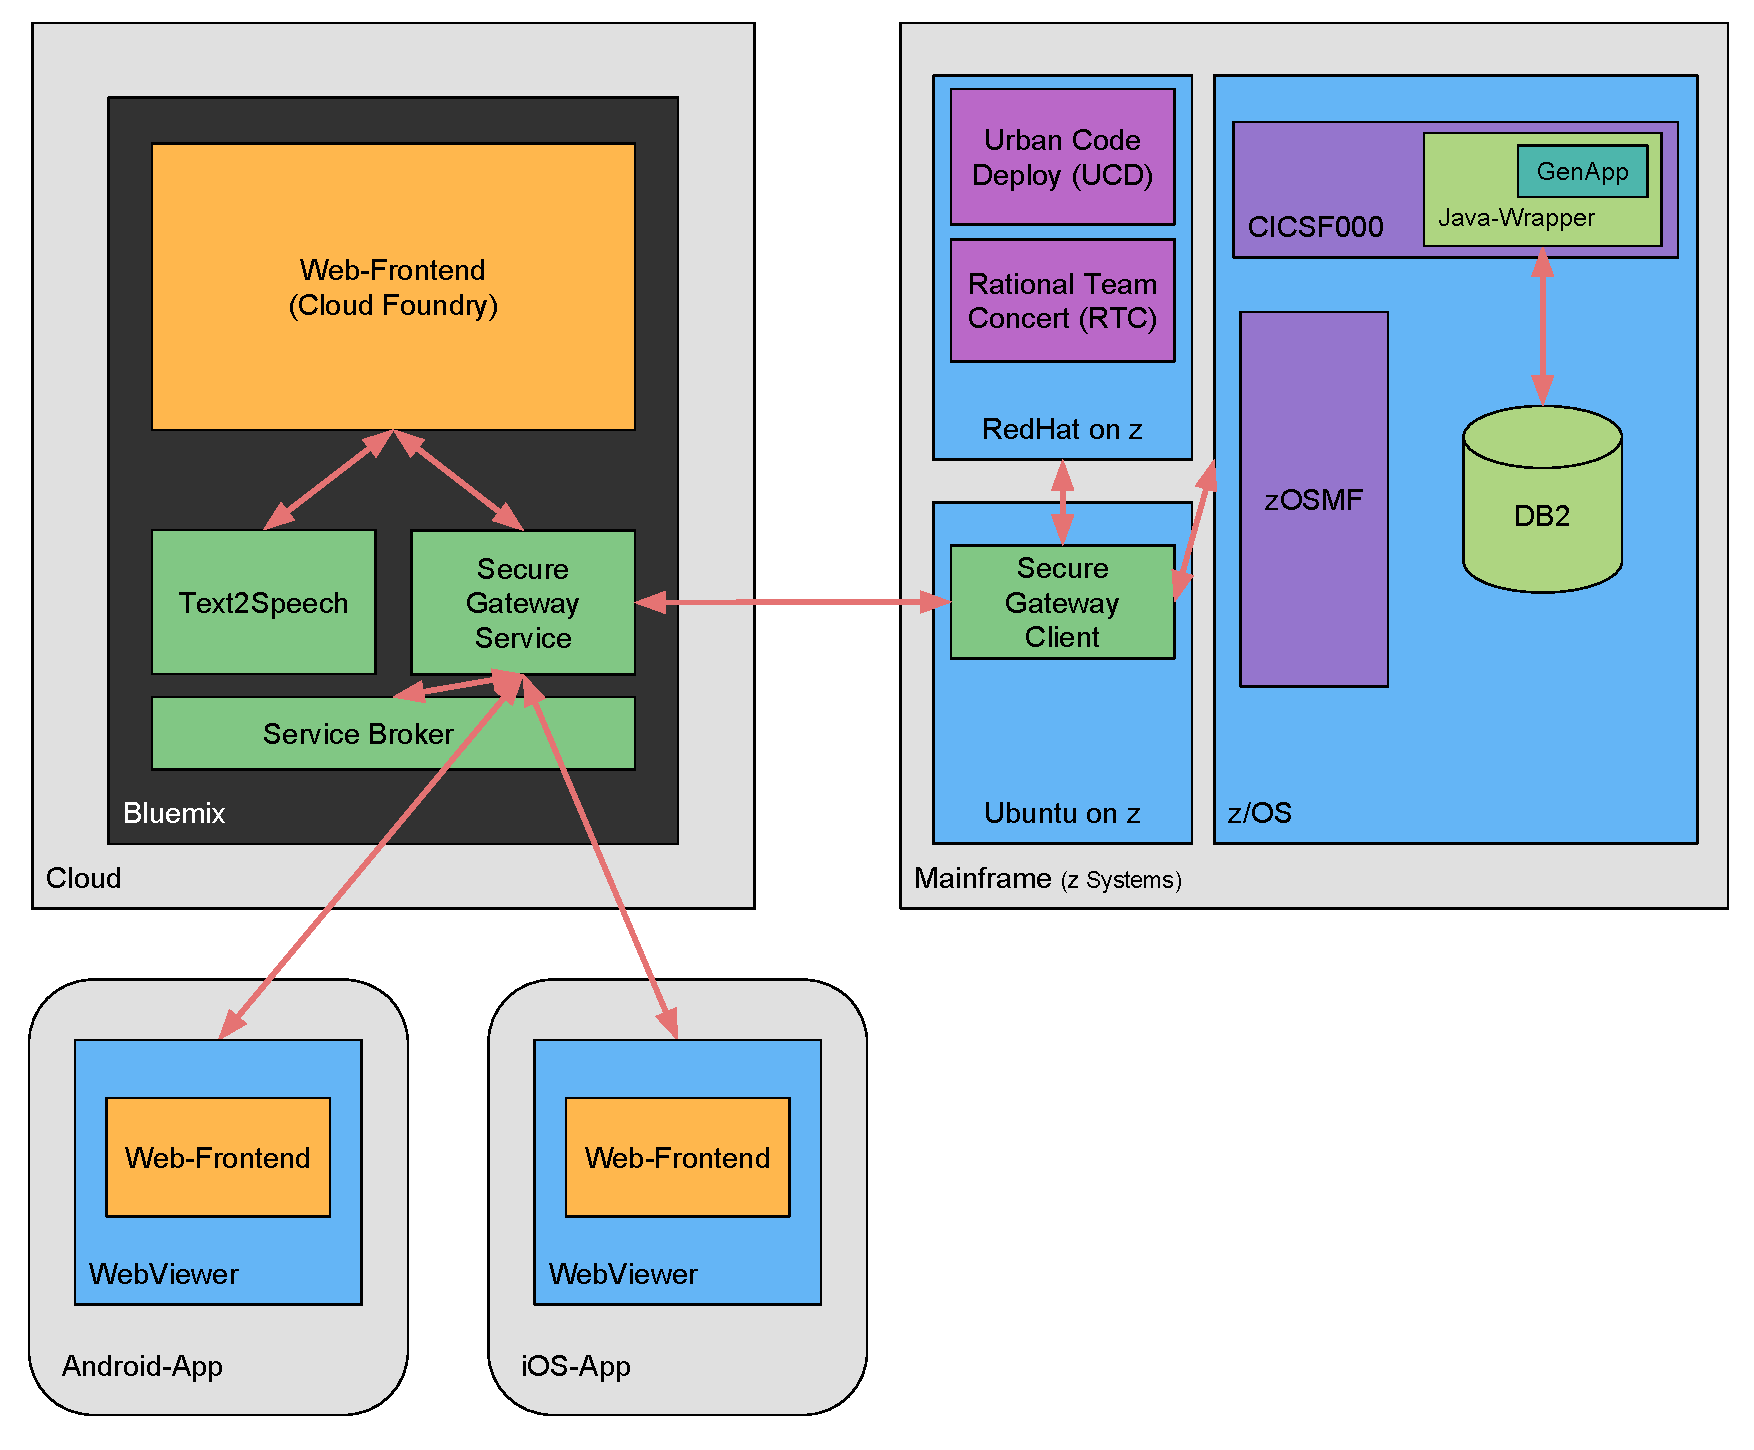
\includegraphics[scale=0.5]{images/kapitel_4/architektur_gesamt.pdf}
  \caption{Gesamtübersicht der Anwendung}
  \label{fig:architektur_gesamtf}
\end{figure}